\documentclass[11pt]{article}
\usepackage{latexsym}
\usepackage{amsmath}
\usepackage{amssymb}
\usepackage{amsthm}
\usepackage{epsfig}
\usepackage{array}
\usepackage[tight]{subfigure}

\usepackage{amsmath}
\DeclareMathOperator*{\argmax}{arg\,max}

\DeclareMathOperator*{\minimize}{min}
\DeclareMathOperator*{\maximize}{max}

\usepackage{algorithm}
 %on linux you may need to run sudo apt-get install texlive-full to install algorithm.sys
\usepackage{algorithmic}

\usepackage{verbatim}

\newcommand{\handout}[5]{
  \noindent
  \begin{center}
  \framebox{
    \vbox{
      \hbox to 5.78in { {#1} \hfill #2 }
      \vspace{4mm}
      \hbox to 5.78in { {\Large \hfill #5  \hfill} }
      \vspace{2mm}
      \hbox to 5.78in { {\em #3 \hfill #4} }
    }
  }
  \end{center}
  \vspace*{4mm}
}

\newcommand{\lecture}[5]{\handout{#1}{#2}{#3}{#4}{#5}}
\newcommand{\collision}[0]{\mathrm{collision}}
\newcommand{\nocollision}[0]{\overline{\collision}}

\newcommand*{\QED}{\hfill\ensuremath{\square}}

\newtheorem{theorem}{Theorem}
\newtheorem{corollary}[theorem]{Corollary}
\newtheorem{lemma}[theorem]{Lemma}
\newtheorem{observation}[theorem]{Observation}
\newtheorem{proposition}[theorem]{Proposition}
\newtheorem{definition}[theorem]{Definition}
\newtheorem{claim}[theorem]{Claim}
\newtheorem{fact}[theorem]{Fact}
\newtheorem{assumption}[theorem]{Assumption}
\newtheorem{note}[theorem]{Note}

% 1-inch margins, from fullpage.sty by H.Partl, Version 2, Dec. 15, 1988.
\topmargin 0pt
\advance \topmargin by -\headheight
\advance \topmargin by -\headsep
\textheight 8.9in
\oddsidemargin 0pt
\evensidemargin \oddsidemargin
\marginparwidth 0.5in
\textwidth 6.5in

\parindent 0in
\parskip 1.5ex
%\renewcommand{\baselinestretch}{1.25}

\begin{document}

\lecture{Statistical Techniques in Robotics (16-831, S20)}{Lecture \#05
  (Wednesday, February 2)}{Lecturer: Kris Kitani}{Scribes: Rachel Zheng, Indraneel Patil}{Online Linear Classification}

\section{Review}


%This section serves as a review of the previous lecture and any other context required to frame the content of the current lecture. 

%You may format the scribes in any way you like, aside from changing font style, size and page format. Please use subsections and paragraphs to increase the readability of your notes.

%Length requirement 1-2 pages.
\subsection{Why do we use regret instead of a loss function in online learning?}
A few reasons discussed in class are outlined here:
\begin{enumerate}
    \item In online learning, the environment can change so it renders the loss function meaningless
    \item The hypothesis functions inside the hypothesis class have limits to performance and none of them achieve perfect performance in the real world
    \item Using a loss function is like comparing yourself against the perfect hypothesis but that doesn't exist
    \item So using regret makes more sense (as a perfect hypothesis does not exist) by instead comparing your performance to the best known hypothesis
\end{enumerate}

\subsection{Prediction with Expert Advice}
The prediction with expert advice problem was first tackled with algorithms like the Greedy algorithm, Halving majority algorithm and their variants which all assumed perfect realizability. Recall that realizability is the assumption that the learner has access to the perfect hypothesis. If this assumption is removed those algorithms break.

In the previous lecture we finished performance analysis for two algorithms which removed this realizability assumption. 
\begin{enumerate}
    \item The Weighted Majority Algorithm
    \item Randomized Weighted Majority Algorithm
\end{enumerate}

\subsection{Some key takeaways}
\begin{enumerate}
    \item The growth of regret for the Weighted Majority Algorithm is linear and is O(t)
    \item Adding randomisation improves performance and reduces regret. The randomised weighted majority algorithm turns out to be "no regret" algorithm using a smart adaptive penalty parameter
    \item Randomised Weighted Majority algorithm is a general algorithm which extends beyond PWEA and can be applied to a wide variety of contexts from classification to matrix games.
    
\end{enumerate}

\section{Online Linear Classification}
\subsection{Problem Setup}
Consider an autonomous inspection system which automatically classifies oranges based on some features into two classes, one for export and the other for the local market. Input to the system are some features of the oranges collected using its sensors. Humans are available to label classes for some oranges. Output of the system should be a class for the oranges (In our case a binary classification of export or local). Such a scenario is ideal for Online linear classification. The system should learn from humans in a "supervised learning way". Online linear classification overlaps with supervised learning and is a type of sampled feedback algorithm. The goal of the overall system is to reach human level performance through online learning.

\begin{enumerate}
    \item Input : feature vector of oranges $x^{(t)}$
    \item Output : Binary Classification  $\hat{y}^{(t)}$
    \item Goal : Learn weights of the classifier
\end{enumerate}

\subsection{Linear classification}

Linear classification algorithms design a hyperplane in the high dimensional feature space and use a prediction rule based on this hyperplane to output a class for  the input. \\
\textbf{What is a hyperplane?} \\
In geometry, a hyperplane is a subspace whose dimension is one less than that of its ambient space (in our case the feature space) and it divides this ambient space into two have spaces. \\
For a 3D feature space, the hyperplanes are 2d planes. \\
For a 2D feature space, the hyperplane is a 1D line.\\
Hyperplanes can be more formally defined as :
$$w\cdot x, w \in \mathbb{R}_+^N, x \in \mathbb{R}_+^N$$
General prediction rule for binary classification :
$$ y = sign(w\cdot x - N) $$


\subsection{Perceptron Algorithm vs Winnow Algorithm}

\begin{center}
\begin{tabular}{ | m{3cm} | m{6cm}| m{6cm} | } 
  \hline
  _ & \textbf{Perceptron algorithm} & \textbf{Winnow Algorithm} \\ 
  \hline
  \textbf{Description} & learns weights of the hyperplane & learns set of disjunctive boolean functions \\ 
  \hline
  \textbf{Type of weights} & Can be both positive and negative & Non negative weights \\ 
  \hline
  \textbf{Type of inputs} & $$ x^t \in \mathbb{R}_+^N $$  & $$ x^t \in {0,1}^N $$ \\ 
  \hline
  \textbf{Feature selection} & Uses all features given by nature  & only uses certain subset of features which are useful \\ 
  \hline
  \textbf{Weight initialisation} & All weights set to 0  & All weights set to 1 \\ 
  \hline
  \textbf{Prediction rule} & $$ y^t =sign(w^t\cdot x^t) $$  & $$ y^t =w^t\cdot x^t > N $$ \\
  \hline
\end{tabular}
\end{center}



\section{Perceptron Algorithm}
\subsection{Definition}
Perceptron is a binary linear classifier. It consists of 4 parts: input, weights and bias, summation, and an activation function. \\
The inputs $x_i$ are multiplied by their weights $w_i$, then summed. The weighted sum is then applied to an activation function, which returns the output $y \in \{1, -1\}$.\\
The weights represent a hyperplane in the input space that classifies the data into two parts.
\begin{figure}[H]
  \centering
  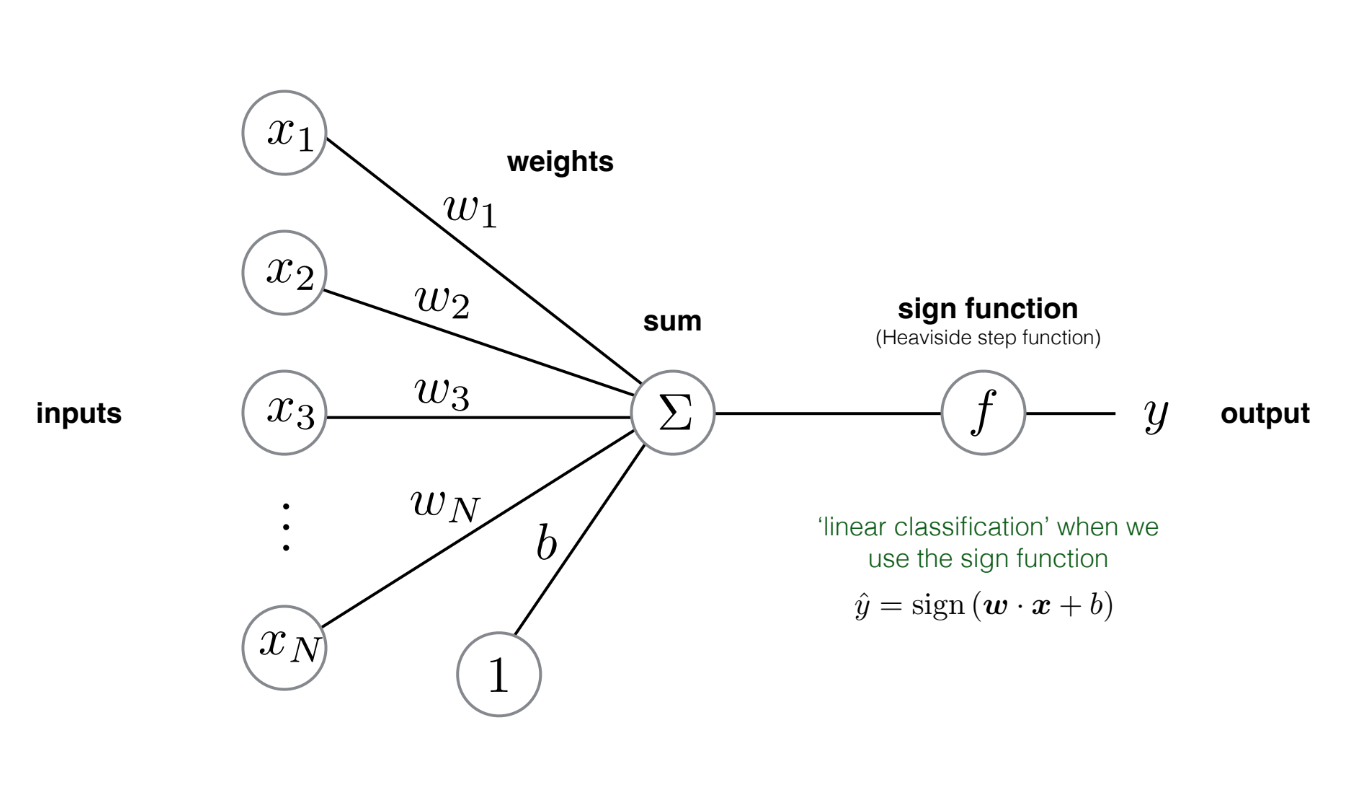
\includegraphics[width=1\linewidth]{perceptron_image.png}
\caption{The Perceptron}
\label{fig:test}
\end{figure}

\subsection{Why do we need the bias term?}
If there is no bias term then the hyperplane will always pass through the origin and fail to learn many classifiers on features which donot split around origin. \\
Bias term introduces an effect of shifting the hyperplane away from the origin in any direction as needed.

\subsection{Types of activation functions}
\begin{enumerate}
    \item \textbf{Identity activation function} : If the activation function is identity then the perceptron algorithm acts like linear regression
    \item \textbf{Sign activation function} : In our case we use this function because we have a linear classification application
\end{enumerate}

\subsection{Algorithm}
The weights are initialized as 0. Then for each time step $t$, we receive the input vector $x^{(t)})$. Then, we predict the output with $\hat{y}^{(t)} = sign(\langle w^{(t)}, x^{(t)} \rangle)$. Next we update the weights. If the prediction was incorrect, then we update according to the rule $w^{(t+1)} = w^{(t)} + y_t x^{(t)}$. If the prediction was correct, we make no changes, so $w^{(t+1)} = w^{(t)}$. The update values of $w$ can become negative.

\begin{algorithm}[H]
\caption{Perceptron Algorithm Pseudocode}
\label{algo:perceptron}
\begin{algorithmic}[1]
\STATE $\boldsymbol{w}^{(0)} \xleftarrow{} 0 $  \hfill $\triangleright$ Weights initialise
\FOR{$t=1,\;\dots,\;T$}
\STATE \textsc{Receive} ($\boldsymbol{x}^{(t)} \in \mathbb{R}^N$) \hfill $\triangleright$ Get input vector
\STATE $\hat{y}^{(t)} = \text{sign} \left( \langle \boldsymbol{w}^{(t-1)}, \boldsymbol{x}^{(t)} \rangle \right)$ \hfill $\triangleright$ Perceptron prediction equation
\STATE \textsc{Receive} ($y^{(t)}\in \{1,-1\}$) \hfill $\triangleright$ Get ground truth
\STATE $\boldsymbol{w}^{(t)} = \boldsymbol{w}^{(t-1)} + y^{(t)} \cdot \boldsymbol{x}^{(t)} \cdot \boldsymbol{1}[y^{(t)}\neq\hat{y}^{(t)}] $ \hfill $\triangleright$ Weight update
\ENDFOR
\end{algorithmic}
\end{algorithm}

The perceptron algorithm is fast since prediction is just a dot product, and update is a sum. However, it is not a large margin classifier since we are only taking into account the sign without any notion of margin. This algorithm also does not work with non-separable data.\\

\subsection{Where does the weight update equation come from?}
As discussed in class, weight update equations have a special connection to the loss function used by the algorithm. Main objective of the weight update step is to decrease the overall loss reported by the loss function. \\
In the case of the perceptron algorithm, we use the \textbf{hinge loss function} which is a common loss function used for training classifiers. The weight update equation comes directly from the gradient of this loss function.

\subsection{Relation between linear separability and realizability}
Recall definition of realizability.  \textbf{Realizability} is the assumption that the learner has access to the perfect hypothesis. \textbf{Linear separability} is the assumption that there exists a linear hyperplane in the feature space which correctly classifies the inputs belonging to different classes into different spaces. \\
In the case of linear classification , realizability and linear separability is one and the same thing. In general they are not the same thing. It is possible that a solution to a problem is realizable but not linearly separable.

\subsection{Mistake Bound}
It can be shown that if the data is linearly separable, then the perceptron algorithm will make a finite number of mistakes.\\
\subsubsection{Potential Function}
First, we define the potential function as the squared L2 norm of the weight vector:
$$\Phi^{(t)} = ||\mathbf{w}^{(t)}||^2 = \sum_n (w_n^{(t)})^2$$
Assuming a mistake was made, we can rewrite the potential function using the update rule
\begin{align*}
    \Phi^{(t)} &= ||\mathbf{w}^{(t-1)}+y^{(t)} \mathbf{x}^{(t)}||^2\\
    &=||\mathbf{w}^{(t-1)}||^2 + ||x^{(t)}||^2 + 2y^{(t)}\langle \mathbf{w}^{(t-1)}, \mathbf{x}^{(t)} \rangle
\end{align*}

\subsubsection{Upper Bound}
We can see that if the learner made a mistake at time $t$, then the term $2y^{(t)}\langle \mathbf{w}^{(t-1)}, \mathbf{x}^{(t)}\rangle$ must be negative since $y^{(t)}$ and $\langle \mathbf{w}^{(t-1)}, \mathbf{x}^{(t)}\rangle$ will have opposite signs. Therefore, we can rewrite as
\begin{align*}
    \Phi^{(t)} &\leq ||\mathbf{w}^{(t-1)}||^2 + ||x^{(t)}||^2\\
    &\leq ||\mathbf{w}^{(t-1)}||^2 + R^2
\end{align*}
Where $R = \max_{t} ||\mathbf{x}^{(t)}||$

We can now find the upper bound using induction.\\
We define the base case as:
$$\Phi^{(1)} \leq ||\mathbf{w}^{(0)}||^2 + R^2$$
For $t>1$, assume the statement is true for $t-1$. When $t=2$:
$$\Phi^{(2)} \leq ||\mathbf{w}^{(0)}||^2 + 2R^2$$
Therefore, for $t=T$:
$$\Phi^{(T)} \leq ||\mathbf{w}^{(0)}||^2 + M^{(T)}R^2$$
The upper bound of the potential function is therefore
\begin{equation}
    \boxed{\Phi^{(T)} \leq M^{(T)}R^2}
\end{equation}

\subsubsection{Lower bound}
To derive the lower bound, we define another potential function, $\langle w^*, w^{(t)}\rangle$, where $w^*$ is the perfect classifier and is a unit vector.\\
Using the property that the dot product between two vectors are the largest when they are oriented in the same direction, 
$$\frac{w}{||w||} = \argmax_{w'}\langle w', w\rangle$$
We derive the upper bound:
Since $w^*$ is a unit vector, the dot product is maximized when
$$\langle w^*, w\rangle \leq \langle \frac{w}{||w||}, w\rangle = \frac{||w||^2}{||w||} = ||w||$$
Therefore, the upper bound is
\begin{equation}
    \boxed{\langle w^*, w^{(T)}\rangle \leq ||w^{(T)}||}
\end{equation}
Next we derive the lower bound:
We apply the update rule to $w^{(t)}$
\begin{align*}
    \langle w^*, w^{(t)}\rangle &= \langle w^*, w^{(t-1)}\rangle + y^{(t)}\langle w^*, x^{(t)}\rangle\\
    &\geq \langle w^*, w^{(t-1)}\rangle + \gamma
\end{align*}
Where $\gamma = \min_t y^{(t)}\langle w^*, x^{(t)}\rangle$, the margin. 
By induction we find
$$\langle w^*, w^{(t)}\rangle \geq \langle w^*, w^{0}\rangle + M^T\cdot \gamma$$
Simplifying
\begin{equation}
    \boxed{\langle w^*, w^{(t)}\rangle \geq M^T\cdot \gamma}
\end{equation}


Combining the upper bound on the dot product (2) and lower bound (3), we can find the lower bound of the potential function:
\begin{equation}
    \boxed{||w^{(T)}||^2 = \Phi^{(T)} \geq (M^{(T)}\cdot \gamma)^2}
\end{equation}


\subsubsection{Combining bounds}
Combining the upper bound (1) and lower bound (4), we finally find the mistake bound:
\begin{equation}
    \boxed{M^T \leq \frac{R^2}{\gamma^2}}
\end{equation}

We see that the mistakes are bounded by $R$, the hyperball that contains all observations, and the margin $\gamma$. Margin represents the degree to which the data is separable. When the margin is large, $M$ decreases. This makes sense because a large margin means our data is highly separable, so there would be less mistakes. When $R$ is large, the $M$ increases. This makes sense because $||x^{(t)}||$ is large, so the weights may be overcorrected. This can result in more mistakes. 

\section{Winnow Algorithm}

We saw the performance of the Perceptron algorithm in the previous section and it works really well under certain assumptions of separability and norm of the data. In other situation the algorithm breaks. The Winnow algorithm improves on this (especially in feature sets where there are a lot of features but some maybe more important than others) by only using a certain subset of features which may be relevant for classification unlike the Perceptron algorithm which uses all the features in the input.

\subsection{Problem setup}

\begin{enumerate}
    \item Input :  $x^{(t)} \in {0,1} $
    \item Output : $\hat{y}^{(t)} = w^{(t)}\cdot x^{(t)} > N$
    \item Assumption : $y=h^*(x)$ (Perfect hypothesis with K features)
\end{enumerate}

\subsection{Missing from the slides}

The weight update rule in the slides is only applied if prediction is wrong and must be repeated for each weight in the input feature space.

\end{document}

